% =====================================================================
%  SAY, ECHO, DO
%  Inverting Institutional and Media Sentiment
%  with Embeddings and Quantitative Finance
%  Technical Report -- Draft v0.2 (readability revision)
% =====================================================================
\documentclass[11pt,a4paper]{article}

% ---------- Packages -------------------------------------------------
\usepackage[utf8]{inputenc}
\IfFileExists{lmodern.sty}{\usepackage[T1]{fontenc}\usepackage{lmodern}}{}
\usepackage[margin=2.6cm]{geometry}
\usepackage{amsmath,amssymb,amsthm,mathtools,bm}
\usepackage{booktabs,tabularx,array}
\usepackage{enumitem}
\usepackage{xcolor}
\usepackage{tikz}
\usetikzlibrary{positioning,arrows.meta,calc,shapes.geometric}
\usepackage{pgfplots}
\pgfplotsset{compat=1.16}
\usepgfplotslibrary{groupplots}
\usepackage[most]{tcolorbox}
\usepackage{titlesec}
\usepackage[numbers,sort&compress]{natbib}
\usepackage{microtype}
\usepackage{setspace}
\usepackage[colorlinks=true,linkcolor=blue!50!black,citecolor=blue!50!black,urlcolor=blue!50!black]{hyperref}
\usepackage[capitalise,noabbrev]{cleveref}

\setstretch{1.15}
\setlength{\parskip}{5pt}
\setlength{\parindent}{0pt}
\setlist{itemsep=3pt,topsep=4pt}

% ---------- Colours --------------------------------------------------
\definecolor{say}{HTML}{8E44AD}
\definecolor{echo}{HTML}{C0392B}
\definecolor{do}{HTML}{1F618D}
\definecolor{price}{HTML}{222222}
\definecolor{good}{HTML}{1E8449}

% ---------- Section style --------------------------------------------
\titleformat{\section}{\Large\bfseries\color{do!80!black}}{\thesection}{0.8em}{}
\titleformat{\subsection}{\large\bfseries}{\thesubsection}{0.7em}{}
\titlespacing*{\section}{0pt}{18pt}{8pt}
\titlespacing*{\subsection}{0pt}{12pt}{5pt}

% ---------- Boxes ----------------------------------------------------
\newtcolorbox{keyidea}[1][Key idea]{enhanced,breakable,colback=do!4,colframe=do!70!black,
  boxrule=0.6pt,arc=2pt,fonttitle=\bfseries\small,title={#1},left=8pt,right=8pt,top=5pt,bottom=5pt}
\newtcolorbox{plainwords}{enhanced,breakable,colback=good!4,colframe=good!60!black,
  boxrule=0pt,leftrule=3pt,arc=0pt,outer arc=0pt,left=8pt,top=4pt,bottom=4pt,
  fontupper=\small,before upper={\textbf{In plain words.}~}}
\newtcolorbox{workedexample}[1]{enhanced,breakable,colback=gray!4,colframe=gray!55!black,
  boxrule=0.6pt,arc=2pt,fonttitle=\bfseries\small,title={Worked example: #1},left=8pt,right=8pt}
\newtcolorbox{techbox}[1]{enhanced,breakable,colback=white,colframe=say!60!black,
  boxrule=0.5pt,arc=2pt,fonttitle=\bfseries\small,coltitle=white,colbacktitle=say!70!black,
  title={Under the hood: #1},left=8pt,right=8pt,fontupper=\small}

% ---------- Theorems -------------------------------------------------
\theoremstyle{plain}
\newtheorem{proposition}{Result}
\theoremstyle{definition}
\newtheorem{definition}{Definition}
\newtheorem{hypothesis}{Hypothesis}
\crefname{proposition}{Result}{Results}
\crefname{hypothesis}{Hypothesis}{Hypotheses}

% ---------- Macros ---------------------------------------------------
\newcommand{\R}{\mathbb{R}}
\newcommand{\E}{\mathbb{E}}
\newcommand{\Prob}{\mathbb{P}}
\newcommand{\N}{\mathcal{N}}
\newcommand{\z}{\bm{z}}
\newcommand{\w}{\bm{w}}
\newcommand{\x}{\bm{x}}
\newcommand{\ind}{\mathbf{1}}
\DeclareMathOperator{\sgn}{sgn}
\DeclareMathOperator{\Var}{Var}
\DeclareMathOperator{\Cov}{Cov}
\newcommand{\SAY}{\textcolor{say}{\textbf{Say}}}
\newcommand{\ECHO}{\textcolor{echo}{\textbf{Echo}}}
\newcommand{\DO}{\textcolor{do}{\textbf{Do}}}

% =====================================================================
\begin{document}

\begin{titlepage}
\centering
\vspace*{2.5cm}
{\Huge\bfseries \textcolor{say}{Say}, \textcolor{echo}{Echo}, \textcolor{do}{Do}\par}
\vspace{0.6cm}
{\Large Inverting Institutional and Media Sentiment\\ with Embeddings and Quantitative Finance\par}
\vspace{1.2cm}
{\large Technical Report --- Draft v0.2\par}
\vspace{0.3cm}
{\normalsize [Author Name] \quad$\cdot$\quad September 2026\par}
\vspace{1.8cm}

\begin{minipage}{0.82\textwidth}
\small
\textbf{Abstract.}
Markets hear three voices. Institutions \emph{say} things in research notes, ratings and interviews. The media \emph{echoes} and amplifies what it hears. Capital \emph{does} things, visible in positioning, order flow and price. Most sentiment models listen only to the first two. This report argues that the tradable signal lives in the \emph{gaps}: between what institutions say and what they do, and between genuinely new information and mere repetition. We build the framework in two halves. The first is an embedding stack that places every document on a \emph{map of meaning}, measures surprise against what was expected, and separates new information from echo using self-exciting point processes. The second is a quantitative stack that recovers hidden positioning from lagged disclosures, measures how much of the narrative the price actually absorbed, and detects whether money moved \emph{before} the narrative turned. A regime model then decides, event by event, whether to follow the story or fade it. We close with a validation protocol designed to make overfitting hard.
\end{minipage}

\vfill
{\footnotesize Draft for discussion. Not investment advice. No empirical results are reported yet; all figures are illustrative and all result tables are templates.\par}
\end{titlepage}

\tableofcontents
\newpage

% =====================================================================
\section{The Idea on One Page}\label{sec:onepage}

Everyone in markets has seen this pattern. A respected bank publishes a gloomy call. Headlines multiply. Social media repeats them. The stock drops, but less than the noise suggests, and a few weeks later it is higher than before. Looking back, the positioning data show that someone was buying all along.

It is tempting to read this as a conspiracy in which institutions frighten the public in order to buy cheaply. Sometimes that happens, and when it does it is illegal. But we do not need to prove intent to trade the pattern. We only need to \emph{measure the disagreement} between three voices:

\begin{center}
\begin{tabular}{@{}>{\raggedright}p{2.0cm}>{\raggedright}p{5.0cm}>{\raggedright\arraybackslash}p{6.2cm}@{}}
\toprule
Voice & What it is & Where we observe it \\
\midrule
\SAY & What institutions publicly claim & Ratings, target changes, strategist notes, management tone on earnings calls, interviews \\
\ECHO & What the media repeats and amplifies & News volume, syndication, social posts, emotional intensity \\
\DO & What capital actually does & Holdings filings, futures positioning, insider trades, options flow, order book, price \\
\bottomrule
\end{tabular}
\end{center}

The framework rests on two inversions.

\begin{keyidea}[The two inversions]
\textbf{1. Read institutions by their deeds, not their words.} When the \SAY\ voice and the \DO\ voice disagree, trust \DO. A bearish institutional call accompanied by institutional buying is a bullish signal.

\textbf{2. Fade the echo, follow the news.} Split media sentiment into a \emph{new-information} part and an \emph{echo} part. Follow the first, since prices tend to drift after real news. Fade the second, since amplification is what overshoots.
\end{keyidea}

The price is the referee. If the story says the stock should fall 6\% and it falls 2\%, someone absorbed the selling. That residual, which we call \emph{absorption}, is often the clearest evidence of what the \DO\ voice is doing.

\begin{figure}[ht]
\centering
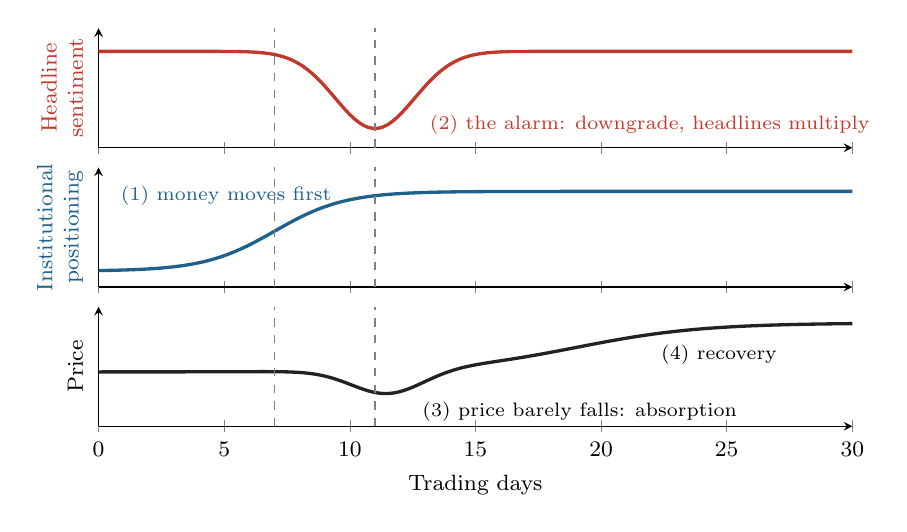
\begin{tikzpicture}
\begin{groupplot}[
  group style={group size=1 by 3, vertical sep=0.25cm, xticklabels at=edge bottom},
  width=0.92\textwidth, height=3.1cm,
  xmin=0, xmax=30, axis lines=left, ytick=\empty,
  xtick={0,5,...,30}, no markers, samples=160, domain=0:30,
  ylabel style={align=center, font=\footnotesize},
  tick label style={font=\footnotesize},
  clip=false]
\nextgroupplot[ylabel={\textcolor{echo}{Headline}\\\textcolor{echo}{sentiment}}, ymin=-1.25, ymax=0.3]
  \addplot[echo, very thick] {-exp(-((x-11)^2)/5)};
  \addplot[gray, dashed] coordinates {(7,-1.25) (7,0.3)};
  \addplot[gray, dashed] coordinates {(11,-1.25) (11,0.3)};
  \node[font=\scriptsize, anchor=west, text=echo] at (axis cs:12.8,-0.95) {(2) the alarm: downgrade, headlines multiply};
\nextgroupplot[ylabel={\textcolor{do}{Institutional}\\\textcolor{do}{positioning}}, ymin=-0.2, ymax=1.3]
  \addplot[do, very thick] {1/(1+exp(-(x-7)/1.4))};
  \addplot[gray, dashed] coordinates {(7,-0.2) (7,1.3)};
  \addplot[gray, dashed] coordinates {(11,-0.2) (11,1.3)};
  \node[font=\scriptsize, anchor=west, text=do] at (axis cs:0.5,0.95) {(1) money moves first};
\nextgroupplot[ylabel={Price}, ymin=95, ymax=106, xlabel={\footnotesize Trading days}]
  \addplot[price, very thick] {100 - 2.2*exp(-((x-11.5)^2)/4) + 4.5/(1+exp(-(x-19)/2.5))};
  \addplot[gray, dashed] coordinates {(7,95) (7,106)};
  \addplot[gray, dashed] coordinates {(11,95) (11,106)};
  \node[font=\scriptsize, anchor=west] at (axis cs:12.5,96.3) {(3) price barely falls: absorption};
  \node[font=\scriptsize, anchor=west] at (axis cs:22,101.6) {(4) recovery};
\end{groupplot}
\end{tikzpicture}
\caption{The pattern we want to detect (stylised, not real data). Positioning builds (1) before the alarm (2). The price falls far less than the alarm implies (3), and then recovers (4). Each numbered step corresponds to a measurable signal in this report.}
\label{fig:pattern}
\end{figure}

The same logic runs in reverse at market tops: euphoric coverage, institutions talking up a name while quietly reducing it, and a price that stalls despite good news. The framework does not hard-code ``always be contrarian''. It decides, event by event, which of four situations we are in (\cref{fig:matrix}).

\begin{figure}[ht]
\centering
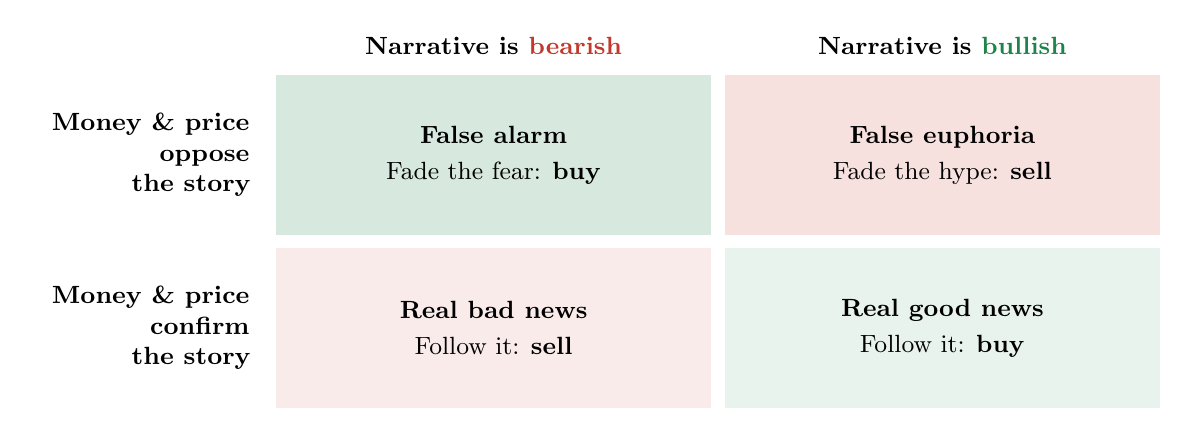
\begin{tikzpicture}[
  cell/.style={draw=white, line width=2pt, minimum width=5.6cm, minimum height=2.1cm, align=center, font=\small},
  head/.style={font=\small\bfseries, align=center}]
\node[cell, fill=good!18] (a) at (0,0) {\textbf{False alarm}\\[2pt] Fade the fear: \textbf{buy}};
\node[cell, fill=echo!15] (b) at (5.7,0) {\textbf{False euphoria}\\[2pt] Fade the hype: \textbf{sell}};
\node[cell, fill=echo!10] (c) at (0,-2.2) {\textbf{Real bad news}\\[2pt] Follow it: \textbf{sell}};
\node[cell, fill=good!10] (d) at (5.7,-2.2) {\textbf{Real good news}\\[2pt] Follow it: \textbf{buy}};
\node[head, above=2pt of a] {Narrative is \textcolor{echo}{bearish}};
\node[head, above=2pt of b] {Narrative is \textcolor{good}{bullish}};
\node[head, left=4pt of a, text width=2.7cm, align=right] {Money \& price\\ \textbf{oppose} the story};
\node[head, left=4pt of c, text width=2.7cm, align=right] {Money \& price\\ \textbf{confirm} the story};
\end{tikzpicture}
\caption{The decision matrix. The narrative alone never determines the trade; its agreement with money and price does.}
\label{fig:matrix}
\end{figure}

% =====================================================================
\section{Why Inverting Sentiment Can Work}\label{sec:why}

\subsection{What the literature already tells us}

The pieces of this idea have strong academic support. Media pessimism predicts short-term price pressure followed by reversal \citep{tetlock2007}. Attention-grabbing news drives buying by less-informed investors \citep{barber2008,da2011}. Noise-trader sentiment can push prices away from value for long periods because arbitrage is risky \citep{delong1990,shleifer1997}. Sophisticated traders can profit by trading against forced or sentiment-driven flow \citep{brunnermeier2005}, and short sellers earn their edge by processing public news better than others \citep{engelberg2012}. Promotional and even fraudulent articles move prices \citep{kogan2023}.

There is also an important counterweight: prices \emph{drift} after genuine headline news and \emph{reverse} after moves with no news \citep{chan2003}. A naive contrarian rule would therefore lose money on real news. Our framework must distinguish the two cases, and that is exactly what the \ECHO\ decomposition (\cref{sec:echo}) and the absorption measure (\cref{sec:absorption}) are for.

\subsection{A tiny model that pins down the signs}

We want theory for one reason: to know \emph{which sign} each signal should have and \emph{why}. A three-line model suffices; the full version and proofs are in \cref{app:model}.

A stock has true value $v$. A public narrative $m = v + \eta$ arrives, where $\eta$ is noise, amplification, or distortion. A crowd moves the price by $\varphi$ per unit of narrative, while an informed trader who knows $v$ trades against mispricing and moves the price by $\lambda$ per unit of flow:
\begin{equation}
  p = \varphi\, m + \lambda\, x, \qquad x = \beta(v - p).
\end{equation}
A rational observer would weight the narrative by $w^\star = \Var(v)/\Var(m)$. The crowd \emph{overreacts} if $\varphi > w^\star$.

\begin{proposition}[When to invert]\label{res:invert}
Future returns load \emph{negatively} on the narrative if and only if the crowd overreacts ($\varphi > w^\star$). If it underreacts, returns drift in the narrative's direction.
\end{proposition}

\begin{proposition}[Absorption reveals the hidden buyer]\label{res:absorb}
The price move \emph{net of} the narrative-implied move, $a = p - \varphi m$, equals the informed trader's impact. It predicts continuation in its own direction: if the price fell less than the story implied, expect it to rise.
\end{proposition}

\begin{proposition}[Watching money always helps]\label{res:money}
Adding any noisy observation of informed positioning strictly reduces forecast error, and it shrinks the weight we need to place on the narrative itself.
\end{proposition}

\begin{plainwords}
Fade the story only when the crowd is overreacting to it. The cleanest evidence of what informed money is doing is how much the price refused to move. Any data on actual positioning makes the forecast sharper.
\end{plainwords}

% =====================================================================
\section{Embeddings: A Map of Meaning}\label{sec:embeddings}

\subsection{The intuition}

An embedding model turns a piece of text into a list of numbers, a point in a high-dimensional space, such that texts with similar meaning land close together. Think of it as a \emph{map of meaning}. Earnings stories form one neighbourhood, merger rumours another, regulatory news a third.

Two properties make this map powerful for finance.
\begin{itemize}
  \item \textbf{Directions carry concepts.} Moving in one direction makes text more fearful; moving in another makes it more hedged or more urgent \citep{park2023}. Sentiment becomes a \emph{projection} onto a direction, not a word count.
  \item \textbf{Distances carry surprise.} If we can predict where on the map the next story \emph{should} land, the distance to where it \emph{does} land measures how surprising it is.
\end{itemize}

\begin{figure}[ht]
\centering
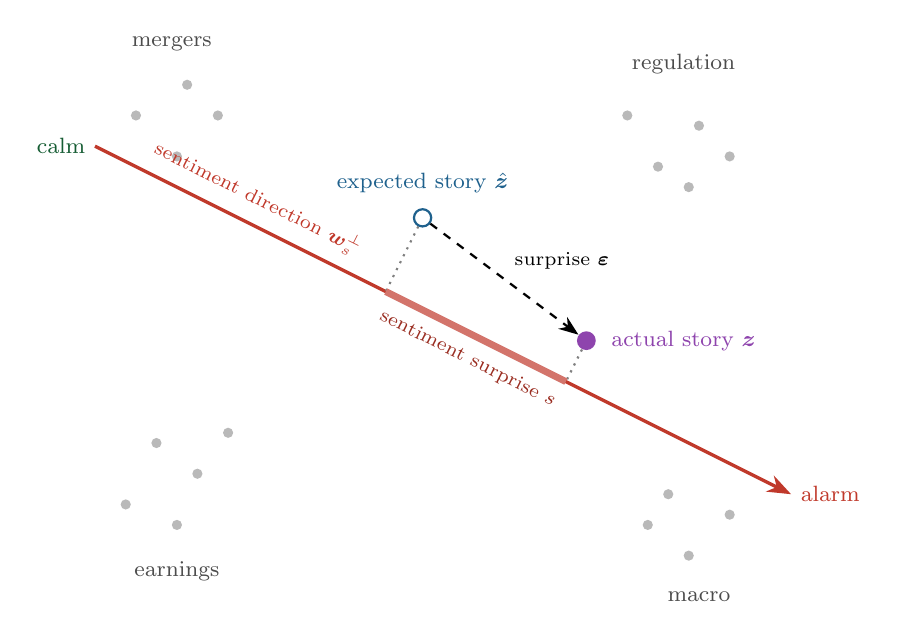
\begin{tikzpicture}[scale=1.3, dot/.style={circle, fill=gray!55, inner sep=1.3pt}]
% clusters
\foreach \p in {(-2.6,-1.3),(-2.2,-1.6),(-2.9,-1.9),(-2.4,-2.1),(-1.9,-1.2)} \node[dot] at \p {};
\node[font=\footnotesize, text=gray!60!black] at (-2.4,-2.55) {earnings};
\foreach \p in {(-2.4,1.5),(-2.0,1.9),(-2.8,1.9),(-2.3,2.2)} \node[dot] at \p {};
\node[font=\footnotesize, text=gray!60!black] at (-2.45,2.6) {mergers};
\foreach \p in {(2.3,1.4),(2.7,1.8),(2.0,1.9),(2.6,1.2),(3.0,1.5)} \node[dot] at \p {};
\node[font=\footnotesize, text=gray!60!black] at (2.55,2.4) {regulation};
\foreach \p in {(2.2,-2.1),(2.6,-2.4),(3.0,-2.0),(2.4,-1.8)} \node[dot] at \p {};
\node[font=\footnotesize, text=gray!60!black] at (2.7,-2.8) {macro};
% sentiment axis through origin, direction (1,-0.5)
\draw[-{Stealth[length=3mm]}, echo, very thick] (-3.2,1.6) -- (3.6,-1.8);
\node[font=\footnotesize, text=echo, anchor=west] at (3.6,-1.8) {alarm};
\node[font=\footnotesize, text=good!70!black, anchor=east] at (-3.2,1.6) {calm};
\node[font=\scriptsize, text=echo, rotate=-26.6, anchor=south] at (-1.7,0.9) {sentiment direction $\w_s^\perp$};
% expected and actual
\node[circle, draw=do, thick, fill=white, inner sep=2.2pt] (ez) at (0,0.9) {};
\node[circle, fill=say, inner sep=2.4pt] (az) at (1.6,-0.3) {};
\node[font=\footnotesize, text=do, anchor=south] at (0,1.05) {expected story $\hat{\z}$};
\node[font=\footnotesize, text=say, anchor=west] at (1.75,-0.3) {actual story $\z$};
\draw[-{Stealth[length=2.5mm]}, dashed, thick] (ez) -- (az) node[midway, above right, font=\scriptsize] {surprise $\bm\varepsilon$};
% projections
\draw[dotted, thick, gray] (ez) -- (-0.36,0.18);
\draw[dotted, thick, gray] (az) -- (1.40,-0.70);
\draw[line width=2.5pt, echo!70] (-0.36,0.18) -- (1.40,-0.70);
\node[font=\scriptsize, text=echo!80!black, rotate=-26.6, anchor=north] at (0.52,-0.32) {sentiment surprise $s$};
\end{tikzpicture}
\caption{The map of meaning (a two-dimensional cartoon of a 1024-dimensional space). Stories cluster by topic. The sentiment direction runs from calm to alarm. Surprise is the gap between where the story was expected to land and where it did; sentiment surprise is the part of that gap along the alarm direction.}
\label{fig:map}
\end{figure}

\subsection{Teaching the map what matters to markets}

Off-the-shelf embeddings organise text by \emph{topic}. Two stories about oil sit together whether they are bullish or bearish. We need a map organised by \emph{economic consequence}.

We fine-tune the encoder with \emph{return-aligned contrastive learning}. For each historical story we record what happened next: abnormal returns at several horizons, abnormal volume, and the change in implied volatility. Stories that led to similar market outcomes are pulled together and others are pushed apart:
\begin{equation}
  \mathcal{L}_{\text{align}} = -\sum_{j}\sum_{k\neq j} q_{jk}\,\log\frac{\exp(\langle\z_j,\z_k\rangle/\tau)}{\sum_{l\neq j}\exp(\langle\z_j,\z_l\rangle/\tau)},
\end{equation}
where $q_{jk}$ is high when stories $j$ and $k$ had similar market aftermaths. A second term keeps the map close to its original semantics so that it does not collapse into a return predictor with no meaning (\cref{app:embeddings}).

\begin{plainwords}
We show the model thousands of past stories and what the market did afterwards, and ask it to place stories with similar aftermaths near each other. The map learns to see ``this kind of news tends to be overdone'' as a location.
\end{plainwords}

\subsection{Directions for fear, hedging and voice}

We estimate several concept directions from labelled examples: \emph{alarm} (urgency, crisis vocabulary), \emph{hedging} (``may'', ``could'', ``risks remain''), \emph{capitulation} (``give up'', ``throw in the towel''), and \emph{voice}, meaning the register of institutional research versus retail commentary.

A subtle problem is that bad news in banking and bad news in energy point in different directions because the topics differ. We remove the topic component so that sentiment is comparable across sectors:
\begin{equation}
  \w_s^\perp = (I - UU^\top)\,\w_s,
\end{equation}
where the columns of $U$ span the main topic directions. The sentiment of any document is then the projection $\langle \w_s^\perp, \z\rangle$. To discover concepts we did not think of, we also train a sparse autoencoder that breaks embeddings into a dictionary of interpretable features \citep{cunningham2023,bricken2023}.

\subsection{Surprise: measuring against expectations, not against zero}

A negative headline that everyone expected carries little information. What moves prices is the \emph{unexpected} part. We train a small sequence model that reads the recent stories about a company, together with its market state, and predicts the embedding of the next story, $\hat\z$. The surprise is
\begin{equation}
  \bm\varepsilon = \z - \hat\z, \qquad
  S = \bm\varepsilon^\top \hat\Sigma^{-1}\bm\varepsilon, \qquad
  s = \langle \w_s^\perp, \bm\varepsilon\rangle .
\end{equation}
$S$ measures \emph{how unexpected} the story is in any direction, while $s$ measures \emph{how much more alarming} it is than expected (\cref{fig:map}).

\begin{plainwords}
We score news on how much worse or better it is than what the market was bracing for, not on how negative it sounds.
\end{plainwords}

\subsection{Echo versus new information}\label{sec:echo}

This is the heart of the media inversion. When one story appears and forty copies follow, the forty copies add attention but no information. We model the arrival of stories in a semantic cluster as a \emph{self-exciting} (Hawkes) process \citep{hawkes1971,bacry2015}, in which each story raises the short-term chance of more stories:
\begin{equation}
  \lambda(t) = \underbrace{\mu}_{\text{new events}} + \underbrace{\sum_{\tau_j<t}\alpha\,e^{-\beta(t-\tau_j)}}_{\text{stories triggered by stories}} .
\end{equation}
A useful property of this model is that it tells us, for each story $j$, the probability that it was \emph{new} rather than \emph{triggered}:
\begin{equation}
  p^{\text{new}}_j = \frac{\mu}{\lambda(\tau_j)}.
\end{equation}
This lets us split any sentiment total cleanly:
\begin{equation}
  s^{\text{new}} = \sum_j p^{\text{new}}_j\, s_j, \qquad
  s^{\text{echo}} = \sum_j \big(1 - p^{\text{new}}_j\big)\, s_j .
\end{equation}

\begin{keyidea}[{The media inversion, made precise}]
Follow $s^{\text{new}}$ and fade $s^{\text{echo}}$. The ratio $\alpha/\beta$, called the \emph{branching ratio}, tells us what share of the coverage is echo. When it approaches one, the narrative is feeding on itself.
\end{keyidea}

We add two supporting measures. \emph{Novelty} is the distance from a new story to its nearest historical neighbours on the map. \emph{Story drift} measures how far the whole cloud of stories about a company has moved over a month, using optimal transport between the two clouds \citep{cuturi2013}.

% =====================================================================
\section{The Institutional Inversion: Say versus Do}\label{sec:saydo}

\subsection{Matching words to deeds}

The \SAY\ voice is easy to observe. The \DO\ voice is harder because it is disclosed late and at different frequencies. The most informative comparisons match the \emph{same kind of actor} on both sides:

\begin{center}
\small
\begin{tabularx}{\textwidth}{@{}lXX@{}}
\toprule
Actor & \SAY & \DO \\
\midrule
Company management & Tone on the earnings call & Insider purchases and sales (Form 4, within two business days) \\
Large asset managers & Public outlooks, interviews & Quarterly holdings (13F, up to 45 days late) \\
Futures market participants & Published macro and commodity views & Weekly positioning by trader category (COT) \\
The market as a whole & Analyst ratings and target changes & Options flow, skew, ETF flows, short interest \\
\bottomrule
\end{tabularx}
\end{center}

For each actor $e$ and stock $i$ we standardise both sides and define the gap
\begin{equation}
  G_{e,i,t} = \widetilde{\text{Say}}_{e,i,t} - \widetilde{\text{Do}}_{e,i,t}, \qquad
  G_{i,t} = \sum_e c_e\, G_{e,i,t},
\end{equation}
where $c_e$ is a credibility weight (\cref{sec:credibility}). A strongly \emph{negative} gap means ``they talk bearish but act bullish'', which is a buy signal. So the institutional inversion trades on $-G$.

\begin{plainwords}
If a CEO sounds worried on the call but directors buy shares the following week, believe the purchases. If strategists sound confident while their category of investor is cutting exposure, believe the cutting.
\end{plainwords}

\subsection{Recovering hidden positioning}

Positioning data are messy: holdings arrive quarterly and weeks late, futures positioning weekly, insider trades within days, options flow in real time. We combine them with a \emph{state-space model}. There is a hidden daily quantity, informed net demand $P_t$, that evolves smoothly, and each data source is a noisy, delayed snapshot of it:
\begin{equation}
  P_t = \rho\, P_{t-1} + \text{shock}_t, \qquad
  y^{(k)}_t = h_k\, P_{t-\ell_k} + \text{noise}^{(k)}_t \quad \text{(only on release dates)} .
\end{equation}
A Kalman filter produces the best current estimate of $P_t$ and, crucially, \emph{how uncertain} that estimate is. When only old quarterly data are available, uncertainty is high and the signal is automatically down-weighted. Recursions are in \cref{app:quant}.

\subsection{A credibility ledger for every source}\label{sec:credibility}

Not all voices deserve equal weight. For each source we keep a running record of how often its calls were right, as a Bayesian posterior on its hit rate. Sources that are reliably right get more weight. Sources that are reliably \emph{wrong} are not discarded: their sign is flipped and they enter the contrarian channel. This makes the inversion data-driven rather than ideological.

% =====================================================================
\section{Forecasting How the Market Will Read the News}\label{sec:interpretation}

The same headline can move prices in opposite directions depending on context. Bad news in a strong market can be shrugged off, and the same news in a fragile market can trigger a crash \citep{veronesi1999}. So we forecast the market's \emph{interpretation}, not the headline's tone.

\begin{definition}[Market Interpretation Function]
Given a story's embedding $\z$ and the market state $\bm\zeta$ (recent returns, volatility, positioning, scheduled events), the Market Interpretation Function $\mathcal{M}(\z,\bm\zeta)$ is the probability distribution of the stock's abnormal return over the reaction window.
\end{definition}

\subsection{The d\'ej\`a vu engine}

The most transparent estimator asks a simple question: \emph{when similar stories hit in similar conditions, what happened?} We retrieve the nearest historical stories on the map and average their outcomes, weighting by similarity of story, similarity of market state, and recency:
\begin{equation}
  \hat\mu(\z,\bm\zeta) = \frac{\sum_j k_j\,\mathrm{AR}_j}{\sum_j k_j}, \qquad
  k_j = \underbrace{e^{\langle\z,\z_j\rangle/h}}_{\text{similar story}}\;
        \underbrace{K(\bm\zeta,\bm\zeta_j)}_{\text{similar market}}\;
        \underbrace{e^{-(t-\tau_j)/T}}_{\text{recent}} .
\end{equation}
Only events whose outcome was fully known before today enter the sum.

Two further estimators complement it. A \emph{mixture-density network} outputs a full distribution with several possible readings, since the same news may be ``bad for earnings'' or ``good because it forces rate cuts''. A \emph{retrieval-augmented language model} reads the new story together with its historical analogues and proposes a reaction, but only as an input feature whose value must be proven in testing.

\begin{techbox}{avoiding look-ahead bias in language models}
A pretrained language model may already ``know'' what happened after an event, which inflates backtests \citep{glasserman2023}. We (i) use frozen model versions whose training ended before each test period, (ii) re-run tests with company names and dates masked, (iii) probe whether the model can recall post-event facts, and (iv) report performance separately before and after each model's training cutoff. Only post-cutoff results count as evidence.
\end{techbox}

% =====================================================================
\section{Reading the Price: Absorption and Lead--Lag}\label{sec:absorption}

\subsection{Absorption}

The interpretation function tells us how far the price \emph{should} have moved. Absorption is the standardised difference from how far it \emph{did} move:
\begin{equation}
  A = \frac{\text{actual reaction} - \text{expected reaction}}{\text{typical error}}
    = \frac{\mathrm{AR} - \hat\mu(\z,\bm\zeta)}{\hat\sigma(\z,\bm\zeta)} .
\end{equation}
This is the empirical version of \cref{res:absorb}: positive $A$ after bad news means buyers stepped in.

\subsection{Effort versus result}

Market microstructure gives an independent check. A well-established empirical regularity, the \emph{square-root law} \citep{bouchaud2018}, says that trading a quantity $Q$ moves the price by roughly $\sigma\sqrt{Q/V}$, where $\sigma$ is daily volatility and $V$ is daily volume. If panic selling was heavy but the price barely moved, the ratio
\begin{equation}
  \Psi = \frac{\sigma\sqrt{Q_{\text{sell}}/V}}{|\text{actual move}|}
\end{equation}
is large. The effort was high and the result small, so somebody absorbed the flow.

\subsection{Who moved first?}

The strongest version of the false-alarm pattern has a clear order: money moves, \emph{then} the narrative turns against it (\cref{fig:pattern}). We measure order with a tool from rough-path theory, the \emph{signed area} between two paths \citep{chevyrev2016}:
\begin{equation}
  \mathcal{A}(X,Y) = \tfrac12\int \big(X_u - X_0\big)\,dY_u - \big(Y_u - Y_0\big)\,dX_u .
\end{equation}
It is positive when moves in $X$ tend to come \emph{before} matching moves in $Y$. Setting $X$ to positioning and $Y$ to the negated narrative, a positive value means ``positioning moved first and the story later turned against it''.

\begin{plainwords}
Draw positioning on one axis and gloom on the other, and trace the path over the past month. If the path loops one way, money led the story; if it loops the other way, money followed it. The area of the loop measures how strongly.
\end{plainwords}

% =====================================================================
\section{Putting It Together}\label{sec:together}

\subsection{One score, two inversions}

A transparent composite combines everything built so far:
\begin{equation}
  D_{i,t} =
  \underbrace{\omega_1\, s^{\text{new}}}_{\substack{\text{follow}\\ \text{news}}}
  \;-\;\underbrace{\omega_2\, s^{\text{echo}}}_{\substack{\text{fade}\\ \text{echo}}}
  \;-\;\underbrace{\omega_3\, G}_{\substack{\text{deeds over}\\ \text{words}}}
  \;+\;\underbrace{\omega_4\, A}_{\substack{\text{follow}\\ \text{absorption}}}
  \;+\;\underbrace{\omega_5\, \mathcal{L}}_{\substack{\text{money}\\ \text{led}}} ,
\end{equation}
where $\mathcal{L}$ is the lead--lag area signed by the direction of the positioning change. The weights are fitted only on training data. Each term has the sign that the model in \cref{sec:why} predicts, so an estimated weight with the wrong sign is itself a warning.

\subsection{Which world are we in?}

The composite is a good starting point, but the right weights depend on the situation. We therefore run a hidden Markov model \citep{hamilton1989} with three regimes:

\begin{center}
\small
\begin{tabularx}{\textwidth}{@{}lXl@{}}
\toprule
Regime & Fingerprint & Action \\
\midrule
Informational & Money and price confirm the narrative; high novelty; low echo & Follow \\
Overreaction & High echo; low novelty; no informed opposition & Fade gently \\
Strategic & Money opposes the narrative; money moved first; high absorption & Fade firmly \\
\bottomrule
\end{tabularx}
\end{center}

For every event the model outputs the probability of each regime using only past data. The probability of the strategic regime is the \emph{Strategic Alarm Probability}. The final forecast blends regime-specific models by these probabilities, and adaptive conformal prediction \citep{gibbs2021} wraps it in an interval with guaranteed long-run coverage. A wide interval means a small position.

\begin{workedexample}{a hypothetical downgrade (illustrative numbers)}
\small
\textbf{Before the event.} Over eight trading days, call open interest in a mid-cap stock rises, put skew flattens, and two directors buy shares. The positioning filter moves from $0.0$ to $+1.2$ standard deviations.

\textbf{Day 0.} Two brokers downgrade the stock, citing weaker demand. Coverage jumps from about 15 stories a day to 140.

\begin{tabularx}{\linewidth}{@{}Xr@{}}
\toprule
Measurement & Value \\
\midrule
Sentiment surprise, total & $-2.8\sigma$ \\
\quad of which new information / echo & $-0.5\sigma$ / $-2.3\sigma$ \\
Branching ratio of the cluster & 0.82 \\
Say--Do gap (bearish words, bullish positioning) & $-3.3$ \\
Expected reaction from the interpretation function & $-6.0\% \pm 2.5\%$ \\
Actual two-day reaction & $-1.9\%$ \\
Absorption $A$ & $+1.6$ \\
Effort versus result $\Psi$ & 3.1 \\
Lead--lag: positioning moved first & yes \\
Regime probabilities (Informational / Overreaction / Strategic) & 0.10 / 0.28 / 0.62 \\
20-day forecast, 90\% interval & $+2.4\%$, $[-1.8\%, +6.5\%]$ \\
\bottomrule
\end{tabularx}

\textbf{Reading.} Most of the gloom is echo. Institutions say bearish things while positioning is bullish, and it moved first. The price absorbed about two thirds of the expected drop. The framework reads this as a probable false alarm and takes a long position, sized modestly because the interval still includes losses.
\end{workedexample}

% =====================================================================
\section{From Signal to Portfolio}\label{sec:portfolio}

Good signals are routinely destroyed by poor construction. Four principles guide this layer; the mathematics is in \cref{app:quant}.

\begin{enumerate}
  \item \textbf{Scale by confidence.} Forecasts become expected returns via $\alpha = \mathrm{IC}\times\sigma\times\text{score}$ \citep{grinold2000}, with the information coefficient measured out of sample and shrunk toward zero. Alternatively, views are blended with market-implied returns through Black--Litterman \citep{black1992}, with view uncertainty taken from the conformal intervals.
  \item \textbf{Stay neutral to known factors.} The portfolio is hedged against market, size, value, profitability, investment and momentum exposures \citep{fama2015,carhart1997}, so that returns come from the signal and not from a disguised factor bet.
  \item \textbf{Pay for liquidity honestly.} The optimiser charges spread costs and square-root market impact. Contrarian trades usually \emph{provide} liquidity to panicking sellers, so passive orders are often possible and cheaper.
  \item \textbf{Size conservatively.} Position size uses a fraction (about a third) of the Kelly-optimal amount \citep{kelly1956}, because estimated edges are always overstated. Execution follows an Almgren--Chriss schedule \citep{almgren2001}.
\end{enumerate}

% =====================================================================
\section{How We Will Know If It Works}\label{sec:validation}

Most published trading signals do not survive honest testing \citep{harvey2016}. The protocol below is designed to make self-deception difficult, and it is fixed before any results are seen.

\subsection{Hypotheses}

\begin{center}
\small
\begin{tabularx}{\textwidth}{@{}lXX@{}}
\toprule
& Claim & Test \\
\midrule
H1 & Echo sentiment reverses; new-information sentiment drifts & Opposite-signed coefficients in return regressions at 5, 20 and 60 days \\
H2 & A negative Say--Do gap predicts positive returns & Sorted portfolios; factor-adjusted alphas \\
H3 & Absorption predicts continuation in its own direction & Coefficient on $A$ controlling for sentiment \\
H4 & Events where money moved first earn more & Split on the lead--lag measure \\
H5 & Learned embeddings beat dictionaries, FinBERT and zero-shot LLM scores & Out-of-sample accuracy comparison (Diebold--Mariano, Giacomini--White) \\
H6 & The full strategy survives costs and overfitting checks & Deflated Sharpe $> 0.95$; probability of overfitting $< 0.2$ \\
\bottomrule
\end{tabularx}
\end{center}

The baselines in H5 are the Loughran--McDonald financial dictionary \citep{loughran2011}, FinBERT \citep{araci2019}, and zero-shot language-model scoring \citep{lopezlira2023}.

\subsection{The anti-overfitting checklist}

\begin{itemize}
  \item \textbf{Point-in-time data only.} Every input carries the timestamp at which it became public, and every model is retrained on a rolling schedule using only data available at that date.
  \item \textbf{Purged, combinatorial cross-validation.} The sample is cut into blocks. Training data that overlap the test period are removed, and a gap is left after each test block \citep{lopezdeprado2018}. Testing many block combinations yields a \emph{distribution} of results rather than one lucky number.
  \item \textbf{Deflate for the number of tries.} The Sharpe ratio is deflated for the number of variants tested and for fat tails \citep{bailey2014dsr}, and the probability of backtest overfitting is reported \citep{bailey2017pbo}.
  \item \textbf{Multiple-testing control.} Feature screening controls the false-discovery rate, and any new factor must clear a $t$-statistic of 3 \citep{harvey2016}. The final strategy is compared with its benchmark using the superior predictive ability test \citep{hansen2005}.
  \item \textbf{Placebos.} Shuffling news timestamps, or shifting news earlier than it happened, must destroy the signal. If it does not, something is leaking.
  \item \textbf{Ablations.} Each layer (echo split, Say--Do gap, absorption, lead--lag) is removed in turn to show what it contributes.
\end{itemize}

\subsection{What the results will look like}

\begin{center}
\small
\begin{tabular}{@{}lccccc@{}}
\toprule
Strategy & Net Sharpe & Deflated SR & Overfit prob. & Factor $\alpha$ $t$ & Turnover \\
\midrule
Dictionary baseline & -- & -- & -- & -- & -- \\
FinBERT baseline & -- & -- & -- & -- & -- \\
Zero-shot LLM baseline & -- & -- & -- & -- & -- \\
Media inversion only & -- & -- & -- & -- & -- \\
Institutional inversion only & -- & -- & -- & -- & -- \\
Full framework & -- & -- & -- & -- & -- \\
\bottomrule
\end{tabular}
\end{center}

% =====================================================================
\section{Risks, Limits and Ethics}\label{sec:risks}

\textbf{We measure disagreement, not intent.} The strategic regime means that money and narrative moved in opposite directions in a particular order. It is not evidence that anyone lied, and results must never be presented as accusations against named institutions. Large firms also operate information barriers between research and trading, so a gap between a firm's research and its funds' holdings is a statistical pattern, not proof of coordination.

\textbf{Being early looks like being wrong.} Fear can intensify for weeks before it reverses. Requiring confirmation from absorption and positioning helps, but drawdowns during persistent overreaction are the main risk.

\textbf{Disclosures are stale.} Quarterly holdings describe positions that may already have changed. They act as slow background information, and the filter's uncertainty estimate keeps them from dominating.

\textbf{Signals decay.} Popular sentiment gauges are widely watched. Capacity and crowding must be measured before any capital is committed.

\textbf{Compliance.} The system uses public information and lawful disclosures only. It must never be used to create or spread narratives intended to move prices, which would itself be market manipulation under rules such as SEC Rule 10b-5 and their equivalents elsewhere. Material non-public information, data licensing and model-risk governance require formal controls.

% =====================================================================
\section{Roadmap}\label{sec:roadmap}

\begin{center}
\small
\begin{tabularx}{\textwidth}{@{}llX@{}}
\toprule
Phase & Weeks & Deliverable \\
\midrule
0. Data & 1--4 & Point-in-time news archive, security master, disclosure release calendars \\
1. Baselines & 5--8 & Dictionary, FinBERT and LLM scores; event-study and cross-validation harness \\
2. Map of meaning & 9--14 & Fine-tuned embeddings, concept directions, surprise model, echo split \\
3. Say--Do & 15--20 & Positioning filter, credibility ledger, interpretation function, absorption, lead--lag \\
4. Synthesis & 21--24 & Composite score, regime model, conformal intervals; test H1--H5 \\
5. Portfolio & 25--28 & Optimiser, costs, capacity; test H6 \\
6. Paper trading & 3--6 months & Live operation with frozen models before any capital \\
\bottomrule
\end{tabularx}
\end{center}

The quickest informative experiment needs no deep learning at all: collect extreme negative news days, measure absorption as the gap between the actual move and the average move for similar past events, and check whether high-absorption events outperform over the next 20 days. If that simple test fails on honest data, the rest of the framework should be reconsidered before it is built.

% =====================================================================
\appendix
\section{The Model in Full}\label{app:model}

\textbf{Setup.} $v\sim\N(0,\sigma_v^2)$; narrative $m=v+\eta$ with $\eta\sim\N(0,\sigma_\eta^2)$ independent. Price $p=\varphi m+\lambda x$ with informed flow $x=\beta(v-p)$, $\lambda,\beta>0$. Define $w^\star=\sigma_v^2/(\sigma_v^2+\sigma_\eta^2)$ and $\kappa=1/(1+\lambda\beta)\in(0,1)$.

Solving the fixed point gives $p=(\varphi m+\lambda\beta v)/(1+\lambda\beta)$ and the return $r=v-p=\kappa(v-\varphi m)$.

\textbf{\Cref{res:invert}.} Joint normality gives $\E[v\mid m]=w^\star m$, so $\E[r\mid m]=\kappa(w^\star-\varphi)m$. Since $\kappa>0$, the loading is negative if and only if $\varphi>w^\star$. \hfill$\square$

\textbf{\Cref{res:absorb}.} $a=p-\varphi m=\lambda x=\lambda\beta(v-p)=\lambda\beta r$, so $\E[r\mid a,m]=a/(\lambda\beta)$, which has the sign of $a$. \hfill$\square$

\textbf{\Cref{res:money}.} Let $\hat x=x+\xi$ with $\xi\sim\N(0,\sigma_\xi^2)$ independent, and $\varsigma^2=\Var(r\mid m)=\kappa^2\sigma_v^2\sigma_\eta^2/(\sigma_v^2+\sigma_\eta^2)$. Conditional on $m$, $(r,\hat x)$ is Gaussian with $\Cov(r,\hat x\mid m)=\beta\varsigma^2$ and $\Var(\hat x\mid m)=\beta^2\varsigma^2+\sigma_\xi^2$. Hence
\[
\E[r\mid m,\hat x]=\kappa(w^\star-\varphi)\frac{\sigma_\xi^2}{\beta^2\varsigma^2+\sigma_\xi^2}\,m+\frac{\beta\varsigma^2}{\beta^2\varsigma^2+\sigma_\xi^2}\,\hat x,
\qquad
\Var(r\mid m,\hat x)=\varsigma^2\frac{\sigma_\xi^2}{\beta^2\varsigma^2+\sigma_\xi^2}<\varsigma^2 .
\]
The loading on $m$ shrinks toward zero as positioning becomes more precise. \hfill$\square$

\textbf{Strategic distortion.} If an informed party can push $\eta$ opposite to $v$, the effective $\sigma_\eta^2$ rises and $w^\star$ falls. A crowd that does not adjust $\varphi$ then overreacts more, strengthening \cref{res:invert}. The strategic case differs from simple overreaction in the sign of $\hat x$ relative to $m$ and in timing.

\textbf{Estimating the multiplier.} The contemporaneous reaction coefficient $\varphi_t$ is tracked with a random-walk Kalman filter on event reactions, and $w^\star_t$ by regressing later fundamental outcomes (earnings surprises, estimate revisions) on the sentiment surprise. The gap $\hat\varphi_t-\hat w^\star_t$ enters the regime model.

\section{Embedding Details}\label{app:embeddings}

\textbf{Encoder.} A transformer encoder \citep{vaswani2017,reimers2019,wang2022e5} with mean pooling and $\ell_2$ normalisation, $D=1024$, adapted with low-rank adapters of rank 16 \citep{hu2022}. Matryoshka training \citep{kusupati2022} provides nested 64-, 256- and 1024-dimensional prefixes for fast retrieval, density estimation and scoring respectively.

\textbf{Return-aligned contrastive loss.} With post-event response vectors $\bm\rho_j$,
\[
q_{jk}=\frac{\exp(-\|\bm\rho_j-\bm\rho_k\|^2/2b^2)}{\sum_{l\neq j}\exp(-\|\bm\rho_j-\bm\rho_l\|^2/2b^2)} .
\]
The semantic anchor is
\[
\mathcal{L}_{\text{anchor}}=\sum_j\mathrm{KL}\Big(\mathrm{softmax}_k\big(\langle\z^{(0)}_j,\z^{(0)}_k\rangle/\tau\big)\,\Big\|\,\mathrm{softmax}_k\big(\langle\z_j,\z_k\rangle/\tau\big)\Big),
\]
where $\z^{(0)}$ comes from the frozen encoder. The objective is $\mathcal{L}_{\text{align}}+\mu_a\mathcal{L}_{\text{anchor}}$, trained only on events whose outcome window closed before the refit date, with $\tau=0.05$ and $\mu_a=0.5$ as starting values.

\textbf{Geometry.} Embeddings are whitened, $\bm u=\hat\Sigma_z^{-1/2}(\z-\hat{\bm\mu}_z)$, using a shrinkage covariance \citep{ledoit2004}, to correct the tendency of transformer embeddings to crowd into a narrow cone.

\textbf{Surprise model.} A four-layer causal transformer over the last 32 story embeddings and the market state, trained with a contrastive predictive objective \citep{oord2018} that scores the true next story against negatives.

\textbf{Sparse autoencoder.} $\bm h=\mathrm{ReLU}(W_e(\bm u-\bm b_d)+\bm b_e)$, $\hat{\bm u}=W_d\bm h+\bm b_d$, loss $\|\bm u-\hat{\bm u}\|^2+\lambda_1\|\bm h\|_1$, with a dictionary eight times the embedding width.

\textbf{Story drift.} For decayed clouds $Q_t$ and $Q_{t-\Delta}$ of embeddings, entropic optimal transport $W_\epsilon=\min_{\bm\Pi}\langle\bm\Pi,C\rangle-\epsilon H(\bm\Pi)$ with $C_{jk}=\|\bm u_j-\bm u_k\|^2$ \citep{cuturi2013}. Structural breaks are tested with the kernel maximum mean discrepancy \citep{gretton2012}.

\textbf{Echo split.} Hawkes parameters $(\mu,\alpha,\beta)$ are fitted by maximum likelihood per semantic cluster on trailing data \citep{hawkes1971,bacry2015}. The immigrant probability $p^{\text{new}}_j=\mu/\lambda(\tau_j)$ follows from the branching (cluster) representation of the process.

\section{Quantitative Details}\label{app:quant}

\textbf{Kalman filter.} State $\bm\xi_t=T\bm\xi_{t-1}+\bm\upsilon_t$, observations $\bm y_t=Z_t\bm\xi_t+\bm\epsilon_t$, where $Z_t$ selects only sources released at $t$ and the state is augmented with lags to handle delayed snapshots:
\begin{align*}
\bm\xi_{t\mid t-1}&=T\bm\xi_{t-1\mid t-1}, & \Sigma_{t\mid t-1}&=T\Sigma_{t-1\mid t-1}T^\top+Q,\\
K_t&=\Sigma_{t\mid t-1}Z_t^\top(Z_t\Sigma_{t\mid t-1}Z_t^\top+H_t)^{-1}, & \bm\xi_{t\mid t}&=\bm\xi_{t\mid t-1}+K_t(\bm y_t-Z_t\bm\xi_{t\mid t-1}),
\end{align*}
with $\Sigma_{t\mid t}=(I-K_tZ_t)\Sigma_{t\mid t-1}$. With no release, the update is skipped.

\textbf{Microstructure.} Order-flow imbalance at the top of the book \citep{cont2014}, Kyle's $\lambda$ from regressing intraday price changes on signed volume \citep{kyle1985}, and flow toxicity via VPIN \citep{easley2012}. Options features: 25-delta risk reversal, put/call open interest, and delta-weighted signed flow.

\textbf{Regime model.} Three-state Gaussian hidden Markov model on the vector of signals, with sticky transitions and states identified by sign restrictions. Only \emph{filtered} probabilities are used; smoothed probabilities use future data and are forbidden.

\textbf{Conformal intervals.} Adaptive conformal inference updates the miscoverage level as $\alpha_{t+1}=\alpha_t+\gamma(\alpha-\mathrm{err}_t)$ \citep{gibbs2021,angelopoulos2021}.

\textbf{Portfolio.} Weights solve
\begin{align*}
\max_{\w}\quad & \bm\alpha^\top\w-\tfrac{\gamma}{2}\w^\top\hat\Sigma\w-\sum_i c_i|\Delta w_i|-\sum_i\eta_i\sigma_i\frac{|\Delta w_i|^{3/2}}{\sqrt{V_i}}\\
\text{s.t.}\quad & B^\top\w=\bm 0,\quad \bm 1^\top\w=0,\quad |w_i|\le\bar w,\quad \|\w\|_1\le G,
\end{align*}
where the $3/2$ power integrates square-root impact and $B$ holds factor exposures. The Black--Litterman posterior is $\bm\mu_{\text{BL}}=[(\tau\Sigma)^{-1}+\bm P^\top\Omega^{-1}\bm P]^{-1}[(\tau\Sigma)^{-1}\bm\Pi+\bm P^\top\Omega^{-1}\bm Q]$ with $\Omega$ from conformal widths. Almgren--Chriss execution follows $X(t)=X_0\sinh(\kappa(T-t))/\sinh(\kappa T)$ with $\kappa=\sqrt{\lambda_{\text{risk}}\sigma^2/\eta}$.

\textbf{Deflated Sharpe ratio.} For an observed Sharpe $\widehat{\mathrm{SR}}$ over $T$ periods, with skewness $\hat\gamma_3$, kurtosis $\hat\gamma_4$, and $M$ trials whose Sharpe ratios have variance $\widehat V$:
\[
\mathrm{DSR}=\Phi\!\left(\frac{(\widehat{\mathrm{SR}}-\mathrm{SR}_0)\sqrt{T-1}}{\sqrt{1-\hat\gamma_3\widehat{\mathrm{SR}}+\frac{\hat\gamma_4-1}{4}\widehat{\mathrm{SR}}^2}}\right),\quad
\mathrm{SR}_0=\sqrt{\widehat V}\Big[(1-\gamma_E)\Phi^{-1}(1-\tfrac1M)+\gamma_E\Phi^{-1}(1-\tfrac{1}{Me})\Big].
\]

\textbf{Cross-validation.} Combinatorial purged cross-validation with $N=10$ blocks and $k=2$ test blocks gives 45 splits and 9 full backtest paths; an embargo at least as long as the forecast horizon follows each test block \citep{lopezdeprado2018}.

\textbf{Event studies.} Abnormal returns from a factor model estimated before the event; standardised tests \citep{boehmer1991} adjusted for cross-correlation of clustered events \citep{kolari2010}; Newey--West errors for overlapping horizons \citep{newey1987}.

% =====================================================================
\section{Glossary}\label{app:glossary}
\begin{center}
\small
\begin{tabularx}{\textwidth}{@{}lX@{}}
\toprule
Term & Meaning \\
\midrule
Embedding & Coordinates of a text on the map of meaning \\
Sentiment surprise $s$ & How much more alarming a story is than expected \\
Echo share & Fraction of coverage triggered by earlier coverage rather than by new events \\
Say--Do gap $G$ & Difference between what an actor says and what it does \\
Interpretation function & Forecast distribution of the market's reaction to a story \\
Absorption $A$ & How much less (or more) the price moved than the story implied \\
Effort versus result $\Psi$ & Expected price impact of the flow compared with the actual move \\
Lead--lag $\mathcal{L}$ & Whether positioning moved before the narrative turned against it \\
Strategic Alarm Probability & Probability that an event belongs to the strategic regime \\
\bottomrule
\end{tabularx}
\end{center}

% =====================================================================
\clearpage
\begin{thebibliography}{99}\small

\bibitem[Almgren and Chriss(2001)]{almgren2001}
Almgren, R., and Chriss, N. (2001). Optimal execution of portfolio transactions. \emph{Journal of Risk}, 3(2), 5--40.

\bibitem[Angelopoulos and Bates(2021)]{angelopoulos2021}
Angelopoulos, A.~N., and Bates, S. (2021). A gentle introduction to conformal prediction and distribution-free uncertainty quantification. arXiv:2107.07511.

\bibitem[Araci(2019)]{araci2019}
Araci, D. (2019). FinBERT: Financial sentiment analysis with pre-trained language models. arXiv:1908.10063.

\bibitem[Bacry et al.(2015)]{bacry2015}
Bacry, E., Mastromatteo, I., and Muzy, J.-F. (2015). Hawkes processes in finance. \emph{Market Microstructure and Liquidity}, 1(1), 1550005.

\bibitem[Bailey et al.(2017)]{bailey2017pbo}
Bailey, D.~H., Borwein, J.~M., L\'opez de Prado, M., and Zhu, Q.~J. (2017). The probability of backtest overfitting. \emph{Journal of Computational Finance}, 20(4), 39--69.

\bibitem[Bailey and L\'opez de Prado(2014)]{bailey2014dsr}
Bailey, D.~H., and L\'opez de Prado, M. (2014). The deflated Sharpe ratio: Correcting for selection bias, backtest overfitting, and non-normality. \emph{Journal of Portfolio Management}, 40(5), 94--107.

\bibitem[Barber and Odean(2008)]{barber2008}
Barber, B.~M., and Odean, T. (2008). All that glitters: The effect of attention and news on the buying behavior of individual and institutional investors. \emph{Review of Financial Studies}, 21(2), 785--818.

\bibitem[Black and Litterman(1992)]{black1992}
Black, F., and Litterman, R. (1992). Global portfolio optimization. \emph{Financial Analysts Journal}, 48(5), 28--43.

\bibitem[Boehmer et al.(1991)]{boehmer1991}
Boehmer, E., Musumeci, J., and Poulsen, A.~B. (1991). Event-study methodology under conditions of event-induced variance. \emph{Journal of Financial Economics}, 30(2), 253--272.

\bibitem[Bouchaud et al.(2018)]{bouchaud2018}
Bouchaud, J.-P., Bonart, J., Donier, J., and Gould, M. (2018). \emph{Trades, Quotes and Prices: Financial Markets Under the Microscope}. Cambridge University Press.

\bibitem[Bricken et al.(2023)]{bricken2023}
Bricken, T., et al. (2023). Towards monosemanticity: Decomposing language models with dictionary learning. \emph{Transformer Circuits Thread}.

\bibitem[Brunnermeier and Pedersen(2005)]{brunnermeier2005}
Brunnermeier, M.~K., and Pedersen, L.~H. (2005). Predatory trading. \emph{Journal of Finance}, 60(4), 1825--1863.

\bibitem[Carhart(1997)]{carhart1997}
Carhart, M.~M. (1997). On persistence in mutual fund performance. \emph{Journal of Finance}, 52(1), 57--82.

\bibitem[Chan(2003)]{chan2003}
Chan, W.~S. (2003). Stock price reaction to news and no-news: Drift and reversal after headlines. \emph{Journal of Financial Economics}, 70(2), 223--260.

\bibitem[Chevyrev and Kormilitzin(2016)]{chevyrev2016}
Chevyrev, I., and Kormilitzin, A. (2016). A primer on the signature method in machine learning. arXiv:1603.03788.

\bibitem[Cont et al.(2014)]{cont2014}
Cont, R., Kukanov, A., and Stoikov, S. (2014). The price impact of order book events. \emph{Journal of Financial Econometrics}, 12(1), 47--88.

\bibitem[Cunningham et al.(2023)]{cunningham2023}
Cunningham, H., Ewart, A., Riggs, L., Huben, R., and Sharkey, L. (2023). Sparse autoencoders find highly interpretable features in language models. arXiv:2309.08600.

\bibitem[Cuturi(2013)]{cuturi2013}
Cuturi, M. (2013). Sinkhorn distances: Lightspeed computation of optimal transport. \emph{Advances in Neural Information Processing Systems}, 26.

\bibitem[Da et al.(2011)]{da2011}
Da, Z., Engelberg, J., and Gao, P. (2011). In search of attention. \emph{Journal of Finance}, 66(5), 1461--1499.

\bibitem[De Long et al.(1990)]{delong1990}
De Long, J.~B., Shleifer, A., Summers, L.~H., and Waldmann, R.~J. (1990). Noise trader risk in financial markets. \emph{Journal of Political Economy}, 98(4), 703--738.

\bibitem[Easley et al.(2012)]{easley2012}
Easley, D., L\'opez de Prado, M., and O'Hara, M. (2012). Flow toxicity and liquidity in a high-frequency world. \emph{Review of Financial Studies}, 25(5), 1457--1493.

\bibitem[Engelberg et al.(2012)]{engelberg2012}
Engelberg, J.~E., Reed, A.~V., and Ringgenberg, M.~C. (2012). How are shorts informed? Short sellers, news, and information processing. \emph{Journal of Financial Economics}, 105(2), 260--278.

\bibitem[Fama and French(2015)]{fama2015}
Fama, E.~F., and French, K.~R. (2015). A five-factor asset pricing model. \emph{Journal of Financial Economics}, 116(1), 1--22.

\bibitem[Gibbs and Cand\`es(2021)]{gibbs2021}
Gibbs, I., and Cand\`es, E. (2021). Adaptive conformal inference under distribution shift. \emph{Advances in Neural Information Processing Systems}, 34.

\bibitem[Glasserman and Lin(2023)]{glasserman2023}
Glasserman, P., and Lin, C. (2023). Assessing look-ahead bias in stock return predictions generated by GPT sentiment analysis. arXiv:2309.17322.

\bibitem[Gretton et al.(2012)]{gretton2012}
Gretton, A., Borgwardt, K.~M., Rasch, M.~J., Sch\"olkopf, B., and Smola, A. (2012). A kernel two-sample test. \emph{Journal of Machine Learning Research}, 13, 723--773.

\bibitem[Grinold and Kahn(2000)]{grinold2000}
Grinold, R.~C., and Kahn, R.~N. (2000). \emph{Active Portfolio Management} (2nd ed.). McGraw-Hill.

\bibitem[Hamilton(1989)]{hamilton1989}
Hamilton, J.~D. (1989). A new approach to the economic analysis of nonstationary time series and the business cycle. \emph{Econometrica}, 57(2), 357--384.

\bibitem[Hansen(2005)]{hansen2005}
Hansen, P.~R. (2005). A test for superior predictive ability. \emph{Journal of Business \& Economic Statistics}, 23(4), 365--380.

\bibitem[Harvey et al.(2016)]{harvey2016}
Harvey, C.~R., Liu, Y., and Zhu, H. (2016). \ldots and the cross-section of expected returns. \emph{Review of Financial Studies}, 29(1), 5--68.

\bibitem[Hawkes(1971)]{hawkes1971}
Hawkes, A.~G. (1971). Spectra of some self-exciting and mutually exciting point processes. \emph{Biometrika}, 58(1), 83--90.

\bibitem[Hu et al.(2022)]{hu2022}
Hu, E.~J., Shen, Y., Wallis, P., Allen-Zhu, Z., Li, Y., Wang, S., Wang, L., and Chen, W. (2022). LoRA: Low-rank adaptation of large language models. \emph{International Conference on Learning Representations}.

\bibitem[Kelly(1956)]{kelly1956}
Kelly, J.~L. (1956). A new interpretation of information rate. \emph{Bell System Technical Journal}, 35(4), 917--926.

\bibitem[Kogan et al.(2023)]{kogan2023}
Kogan, S., Moskowitz, T.~J., and Niessner, M. (2023). Social media and financial news manipulation. \emph{Review of Finance}, 27(4), 1229--1268.

\bibitem[Kolari and Pynn\"onen(2010)]{kolari2010}
Kolari, J.~W., and Pynn\"onen, S. (2010). Event study testing with cross-sectional correlation of abnormal returns. \emph{Review of Financial Studies}, 23(11), 3996--4025.

\bibitem[Kusupati et al.(2022)]{kusupati2022}
Kusupati, A., et al. (2022). Matryoshka representation learning. \emph{Advances in Neural Information Processing Systems}, 35.

\bibitem[Kyle(1985)]{kyle1985}
Kyle, A.~S. (1985). Continuous auctions and insider trading. \emph{Econometrica}, 53(6), 1315--1335.

\bibitem[Ledoit and Wolf(2004)]{ledoit2004}
Ledoit, O., and Wolf, M. (2004). A well-conditioned estimator for large-dimensional covariance matrices. \emph{Journal of Multivariate Analysis}, 88(2), 365--411.

\bibitem[L\'opez de Prado(2018)]{lopezdeprado2018}
L\'opez de Prado, M. (2018). \emph{Advances in Financial Machine Learning}. Wiley.

\bibitem[Lopez-Lira and Tang(2023)]{lopezlira2023}
Lopez-Lira, A., and Tang, Y. (2023). Can ChatGPT forecast stock price movements? Return predictability and large language models. arXiv:2304.07619.

\bibitem[Loughran and McDonald(2011)]{loughran2011}
Loughran, T., and McDonald, B. (2011). When is a liability not a liability? Textual analysis, dictionaries, and 10-Ks. \emph{Journal of Finance}, 66(1), 35--65.

\bibitem[Newey and West(1987)]{newey1987}
Newey, W.~K., and West, K.~D. (1987). A simple, positive semi-definite, heteroskedasticity and autocorrelation consistent covariance matrix. \emph{Econometrica}, 55(3), 703--708.

\bibitem[van den Oord et al.(2018)]{oord2018}
van den Oord, A., Li, Y., and Vinyals, O. (2018). Representation learning with contrastive predictive coding. arXiv:1807.03748.

\bibitem[Park et al.(2023)]{park2023}
Park, K., Choe, Y.~J., and Veitch, V. (2023). The linear representation hypothesis and the geometry of large language models. arXiv:2311.03658.

\bibitem[Reimers and Gurevych(2019)]{reimers2019}
Reimers, N., and Gurevych, I. (2019). Sentence-BERT: Sentence embeddings using Siamese BERT-networks. \emph{Proceedings of EMNLP-IJCNLP}.

\bibitem[Shleifer and Vishny(1997)]{shleifer1997}
Shleifer, A., and Vishny, R.~W. (1997). The limits of arbitrage. \emph{Journal of Finance}, 52(1), 35--55.

\bibitem[Tetlock(2007)]{tetlock2007}
Tetlock, P.~C. (2007). Giving content to investor sentiment: The role of media in the stock market. \emph{Journal of Finance}, 62(3), 1139--1168.

\bibitem[Vaswani et al.(2017)]{vaswani2017}
Vaswani, A., et al. (2017). Attention is all you need. \emph{Advances in Neural Information Processing Systems}, 30.

\bibitem[Veronesi(1999)]{veronesi1999}
Veronesi, P. (1999). Stock market overreaction to bad news in good times: A rational expectations equilibrium model. \emph{Review of Financial Studies}, 12(5), 975--1007.

\bibitem[Wang et al.(2022)]{wang2022e5}
Wang, L., et al. (2022). Text embeddings by weakly-supervised contrastive pre-training. arXiv:2212.03533.

\end{thebibliography}

\end{document}
